\section{Question 4}
In this question we are asked to perform a principle component analysis, plot the eigenspectrum and plot the data projected onto the first two components.
\subsection{Description of software}\label{q4}
I have implemented my own PCA following the method outlined in \cite[chapter~12]{bishop}. Given a data set, without labels, I normalise the data, then calculate the mean for each dimension, then sample the covarience, get the eigenvectors of the covarience, sort the vectors, which allows me to plot the spectrum as well as the principle components.
\subsection{Results}
\begin{minipage}{7cm}
  \centering
  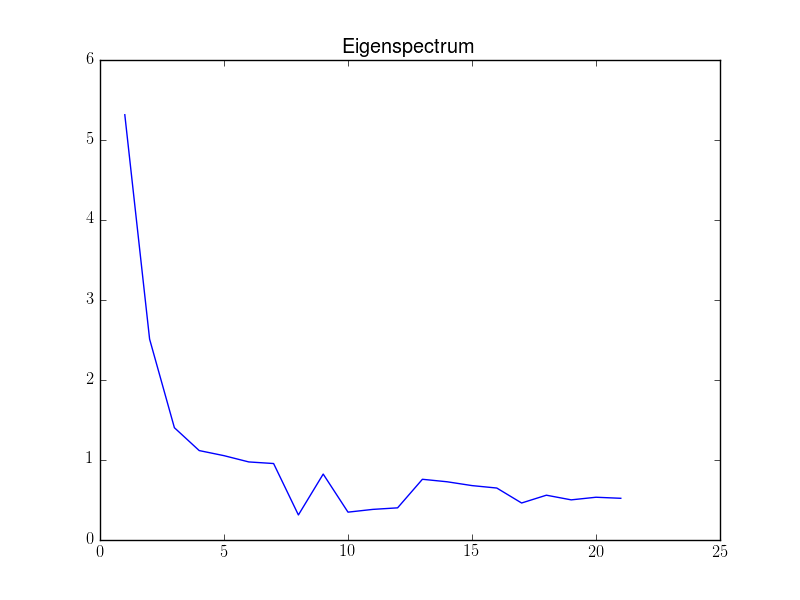
\includegraphics[scale=0.38]{img/eigenspectrum.png}
  \captionof{figure}{Eigenspectrum}
  \label{eigenspectrum}
\end{minipage}
\begin{minipage}{7cm}
  \centering
  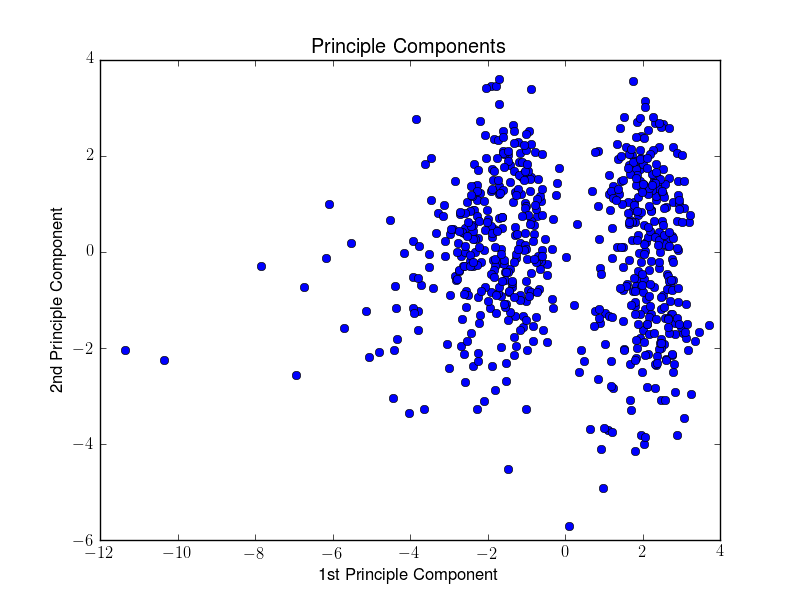
\includegraphics[scale=0.38]{img/components.png}
  \captionof{figure}{The principle components}
  \label{components}
\end{minipage}
